\chapter{The DSDM Lightweight Arm }
\label{sec:ExperimentalValidation}

\vspace{-5pt}
{ \Large Mechanical Design, Control and Software Architecture }

{
\begin{flushright}
\textit{"What I cannot create, I do not understand."} \\ 
\emph{-- Richard Phillips Feynman}
\end{flushright}
}
\vspace{10pt}

%\begin{flushright}
%\small"The test of all knowledge is experiment. Experiment is the sole judge of scientific truth." \\ \emph{Richard Phillips Feynman}
%\end{flushright}


This chapter present a novel 3-DoF robotic arm prototype using DSDM actuators, see Fig. \ref{fig:dsdm_arm_zoom} and Fig. \ref{fig:dsdm_arm}. The mechanical design of the DSDM actuators and the robotic arm is discussed, as well as the control and software implementation.

\begin{figure}[htb]
	\centering
		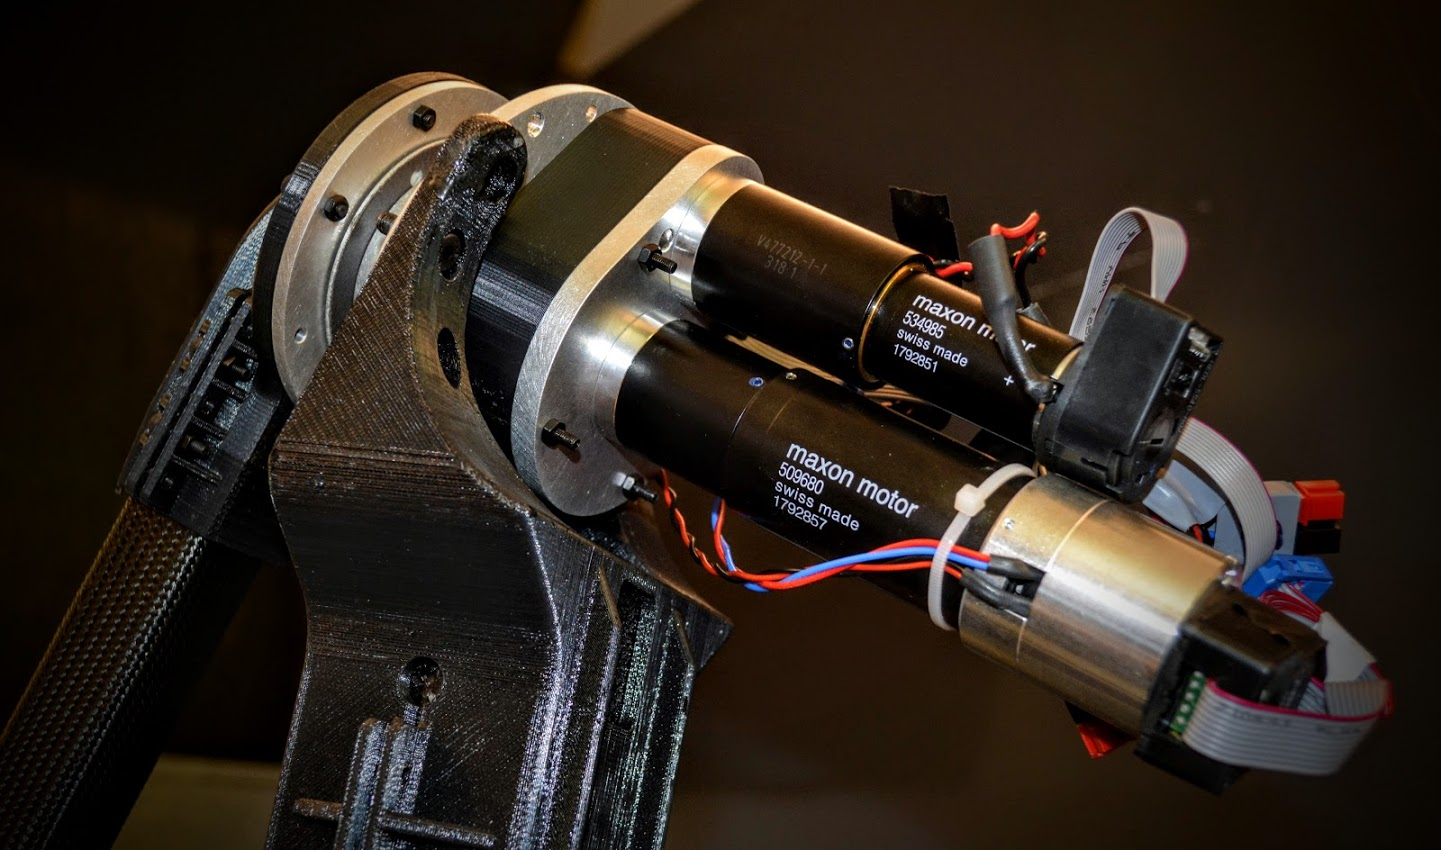
\includegraphics[width=0.70\textwidth]{arm_proto_zoom.jpg}
	\caption{Second joint of the DSDM-Arm}
	\label{fig:dsdm_arm_zoom}
\end{figure}

\begin{figure}[htp]
	\centering
		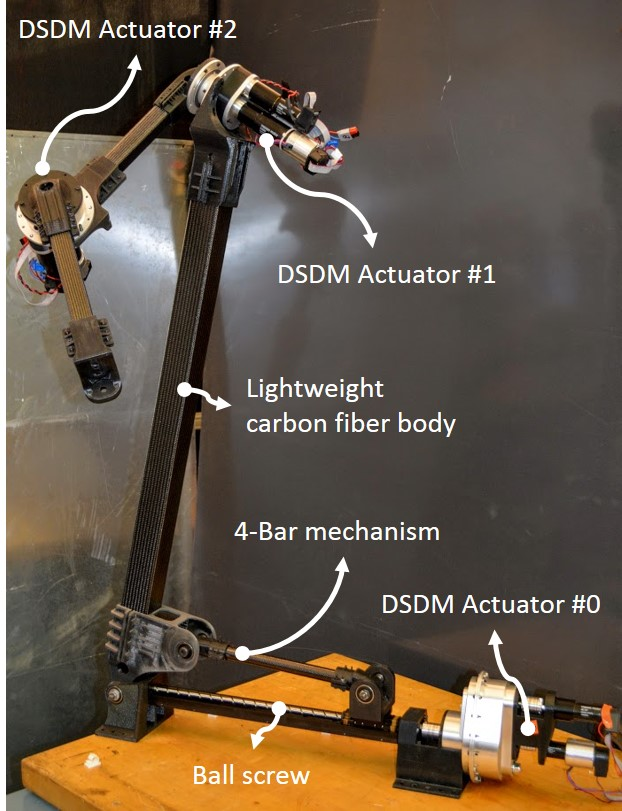
\includegraphics[width=0.95\textwidth]{arm_proto_3.jpg}
	\caption{DSDM-Arm: 3-DoF custom arm using 3 DSDM actuators}
	\label{fig:dsdm_arm}
\end{figure}

\section{Mechanical Design}

This section describe the mechanical design of the arm. The goal was to develop a research platform to validate experimentally the ideas proposed in this thesis, but also to demonstrate the advantage of robotic system with variable gear-ratio actuators. This arm is thus design to be very light-weight compared to robotic arm of similar size, maximum speeds and forces. 

\subsection{DSDM Actuator Design}
\label{sec:ActuatorDesign}
 
Three actuator prototypes were developed for the shoulder, elbow and wrist DoF of the arm, with different mechanical advantages. The shoulder actuator is designed to drive a ballscrew, for a large efficient reduction, and the others actuators are embedded into revolute joints. 

\subsubsection{3-port differential gear-box}

One of the main design challenge arising from the DSDM architecture, is the mechanical implementation of the differential junction between the two motors and the output. In a car powertrain, the differential required to allow a single motor to transmit torque to two wheels rotating at different velocities, is typically implemented with bevel gears. The approach taken here is different, a planetary set of gear is used, where the ring-gear (typically fixed) is mounted on bearing and connected to a parallel shaft. The connection to the parallel shaft is done with a stage of spur gears, with external gear teeth on the ring-gear assembly and another spur gear on the parallel shaft, see Fig. \ref{fig:diff1}. This configuration allows for all the shafts in the transmission and the motors to be parallel, winch simplify the design. In all implementation, the correspondence is given by Table \ref{tab:PlanetaryGearingInputsAndOutput}. This correspondence is picked to match the kinematic relationships arising from sizing constraints in the gearing. From eq. \eqref{eq:kinematic}, with a typical ratio in the planetary of $N=3$ (planet-gear size over internal ring-gear size), and a reduction ratio of $r_2=4$ for the parallel shaft connection (smaller $r_2$ would require large distance between parallel shafts leading to larger transmission volume and larger $r_2$ is difficult to achieve in a single spur-gear stage), it leads to:
%
\begin{align}
	N \approx 3 \quad r_2 \approx 4 \quad\Rightarrow\quad R_1 = N+1 \approx 4 \quad R_2 = r_2 \frac{N+1}{N} \approx 5
\end{align}
%
Hence, the largest reduction through the differential gearing is assigned to M2 and the smallest reduction to M1. This choice is also motivated by the fact that the path going through the ring-gear and the additional stage, would lead to more friction and inertia which is less a concern for high-force mode than for high-speed mode. 

\begin{table}[htbp]
	\centering
		\begin{tabular}{ c c }
			\hline
			Rotating assembly & Role \\
			\hline \hline
			Planet carrier assembly & Actuator output \\
			Parallel shaft (connected to the ring-gear) & Motor M2 input (high-force) \\
			Sun gear shaft          & Motor M1 input (high-speed) \\
			\hline
		\end{tabular}
	\caption{Planetary gearing inputs and output}
	\label{tab:PlanetaryGearingInputsAndOutput}
\end{table}

\begin{figure}[htp]
        \centering
				\subfloat[Linear Actuator]{ % intrinsic dynamics
				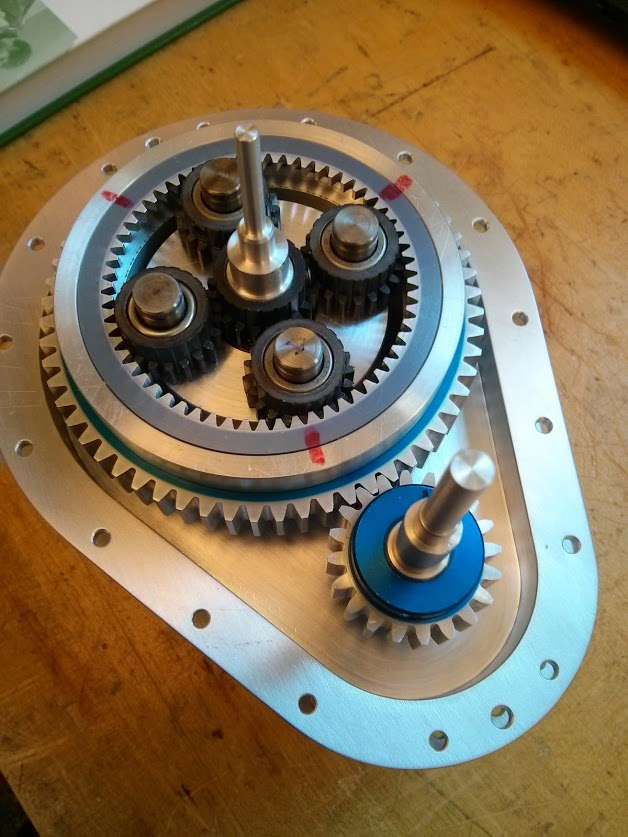
\includegraphics[width=0.40\textwidth]{gears.jpg} 
				\label{fig:diff1}}
				\hspace{+5pt}
        \subfloat[Revolute Joint]{ % intrinsic dynamics
				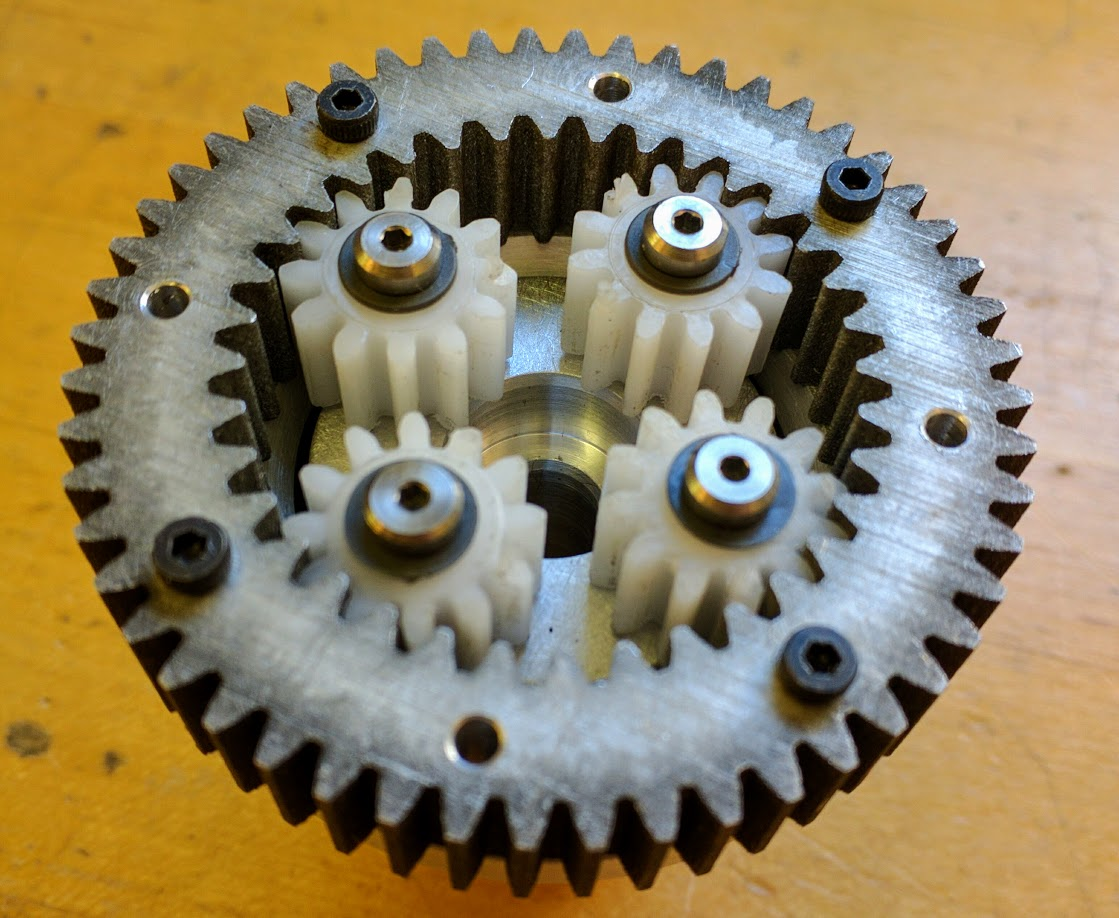
\includegraphics[width=0.50\textwidth]{gears_new.jpg}
				\label{fig:diff2}}
        \caption{Differential gear-box implemented with a planetary}
				\label{fig:differnentials}
\end{figure}

Fig. \ref{fig:diff1} shows the designed differential gearing for the linear actuator prototype and Fig. \ref{fig:diff2} shows the designed differential gearing for the revolute actuators. The first design (a) was using only off-the-shelf gear, which led to a big assembly. For the second design (b) a lot of effort was put into downsizing the assembly. For instance, custom ring gears with both internal and external gear teeth were designed, to minimize the diameter of the ring-gear assembly.

\subsubsection{Brake}

The second challenging mechanical component in a DSDM, is the brake. As discussed in Chapter, \ref{sec:MultipleSpeedActuationTechnology} control schemes can be used to bring M1 velocity to zero before engaging the brake, hence the brake only has to be a locking mechanism and does not have to be able to dissipate power. However, during high-force mode, large holding torque must be sustained. From eq. \eqref{eq:torque}, the holding torque requirement can be computed in term of desired maximum output force during high-force mode, or by the maximum M2 motor torque: 
%
\begin{align}
	\tau_{brake} = \frac{ \operatornamewithlimits{max} \left[ \tau_{output} \right] }{R_1} = \frac{ R_2 }{ R_1 } \operatornamewithlimits{max} \left[  \tau_2 \right]
	\label{eq:brakelim}
\end{align}
%
Hence, the design of the brake is coupled with the desired ratio between $R_1$ and $R_2$. If the high-force mode gear-ratio $R_2$ is 10 times greater than the high-speed mode gear-ratio $R_1$, than the brake must be able to hold torques 10 times greater than M2 output torque. 

Because it allows for simpler and modular designs, it was decided to use off-the-shelf \textit{Maxon} motor brakes that can be mounted directly on a motor assembly. All actuator designs use the \textit{Maxon} motor brake AB-28, which have a holding torque capability of 0.4 Nm and weight 51 g. 


\subsubsection{Revolute Joint Actuators}

Fig. \ref{fig:dsdm_act} shows the prototype for a revolute DSDM actuator. The elbow and wrist actuator have the same design with the exception of using different overall gear-ratios.

\begin{figure}[htp]
	\centering
		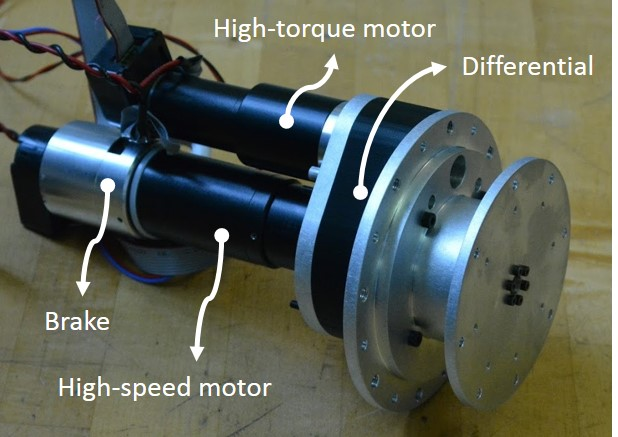
\includegraphics[width=0.70\textwidth]{dsdm_proto_2.jpg}
	\caption{Revolute joint DSDM actuator prototype } %Max continuous torque of 40 Nm and maximum velocity of 100 RPM
	\label{fig:dsdm_act}
\end{figure}

The design for the revolute actuator consist of a custom housing holding both the planetary differential and support bearing for the output. Discrete \textit{Maxon} motors with gear-heads of the serie GP32 can be attached to the back of the gear-box. It is thus possible to attach a wide-range of motor, from 20 watts to 200 watts, and with a wide range of additional gear-head reduction. Fig. \ref{fig:dsdm_section} show the internal architecture of the system with a section view of the CAD model, and Fig. \ref{fig:dsdm_parts} shows all the internal parts of the actuator assembly. 

\begin{figure}[htp]
	\centering
		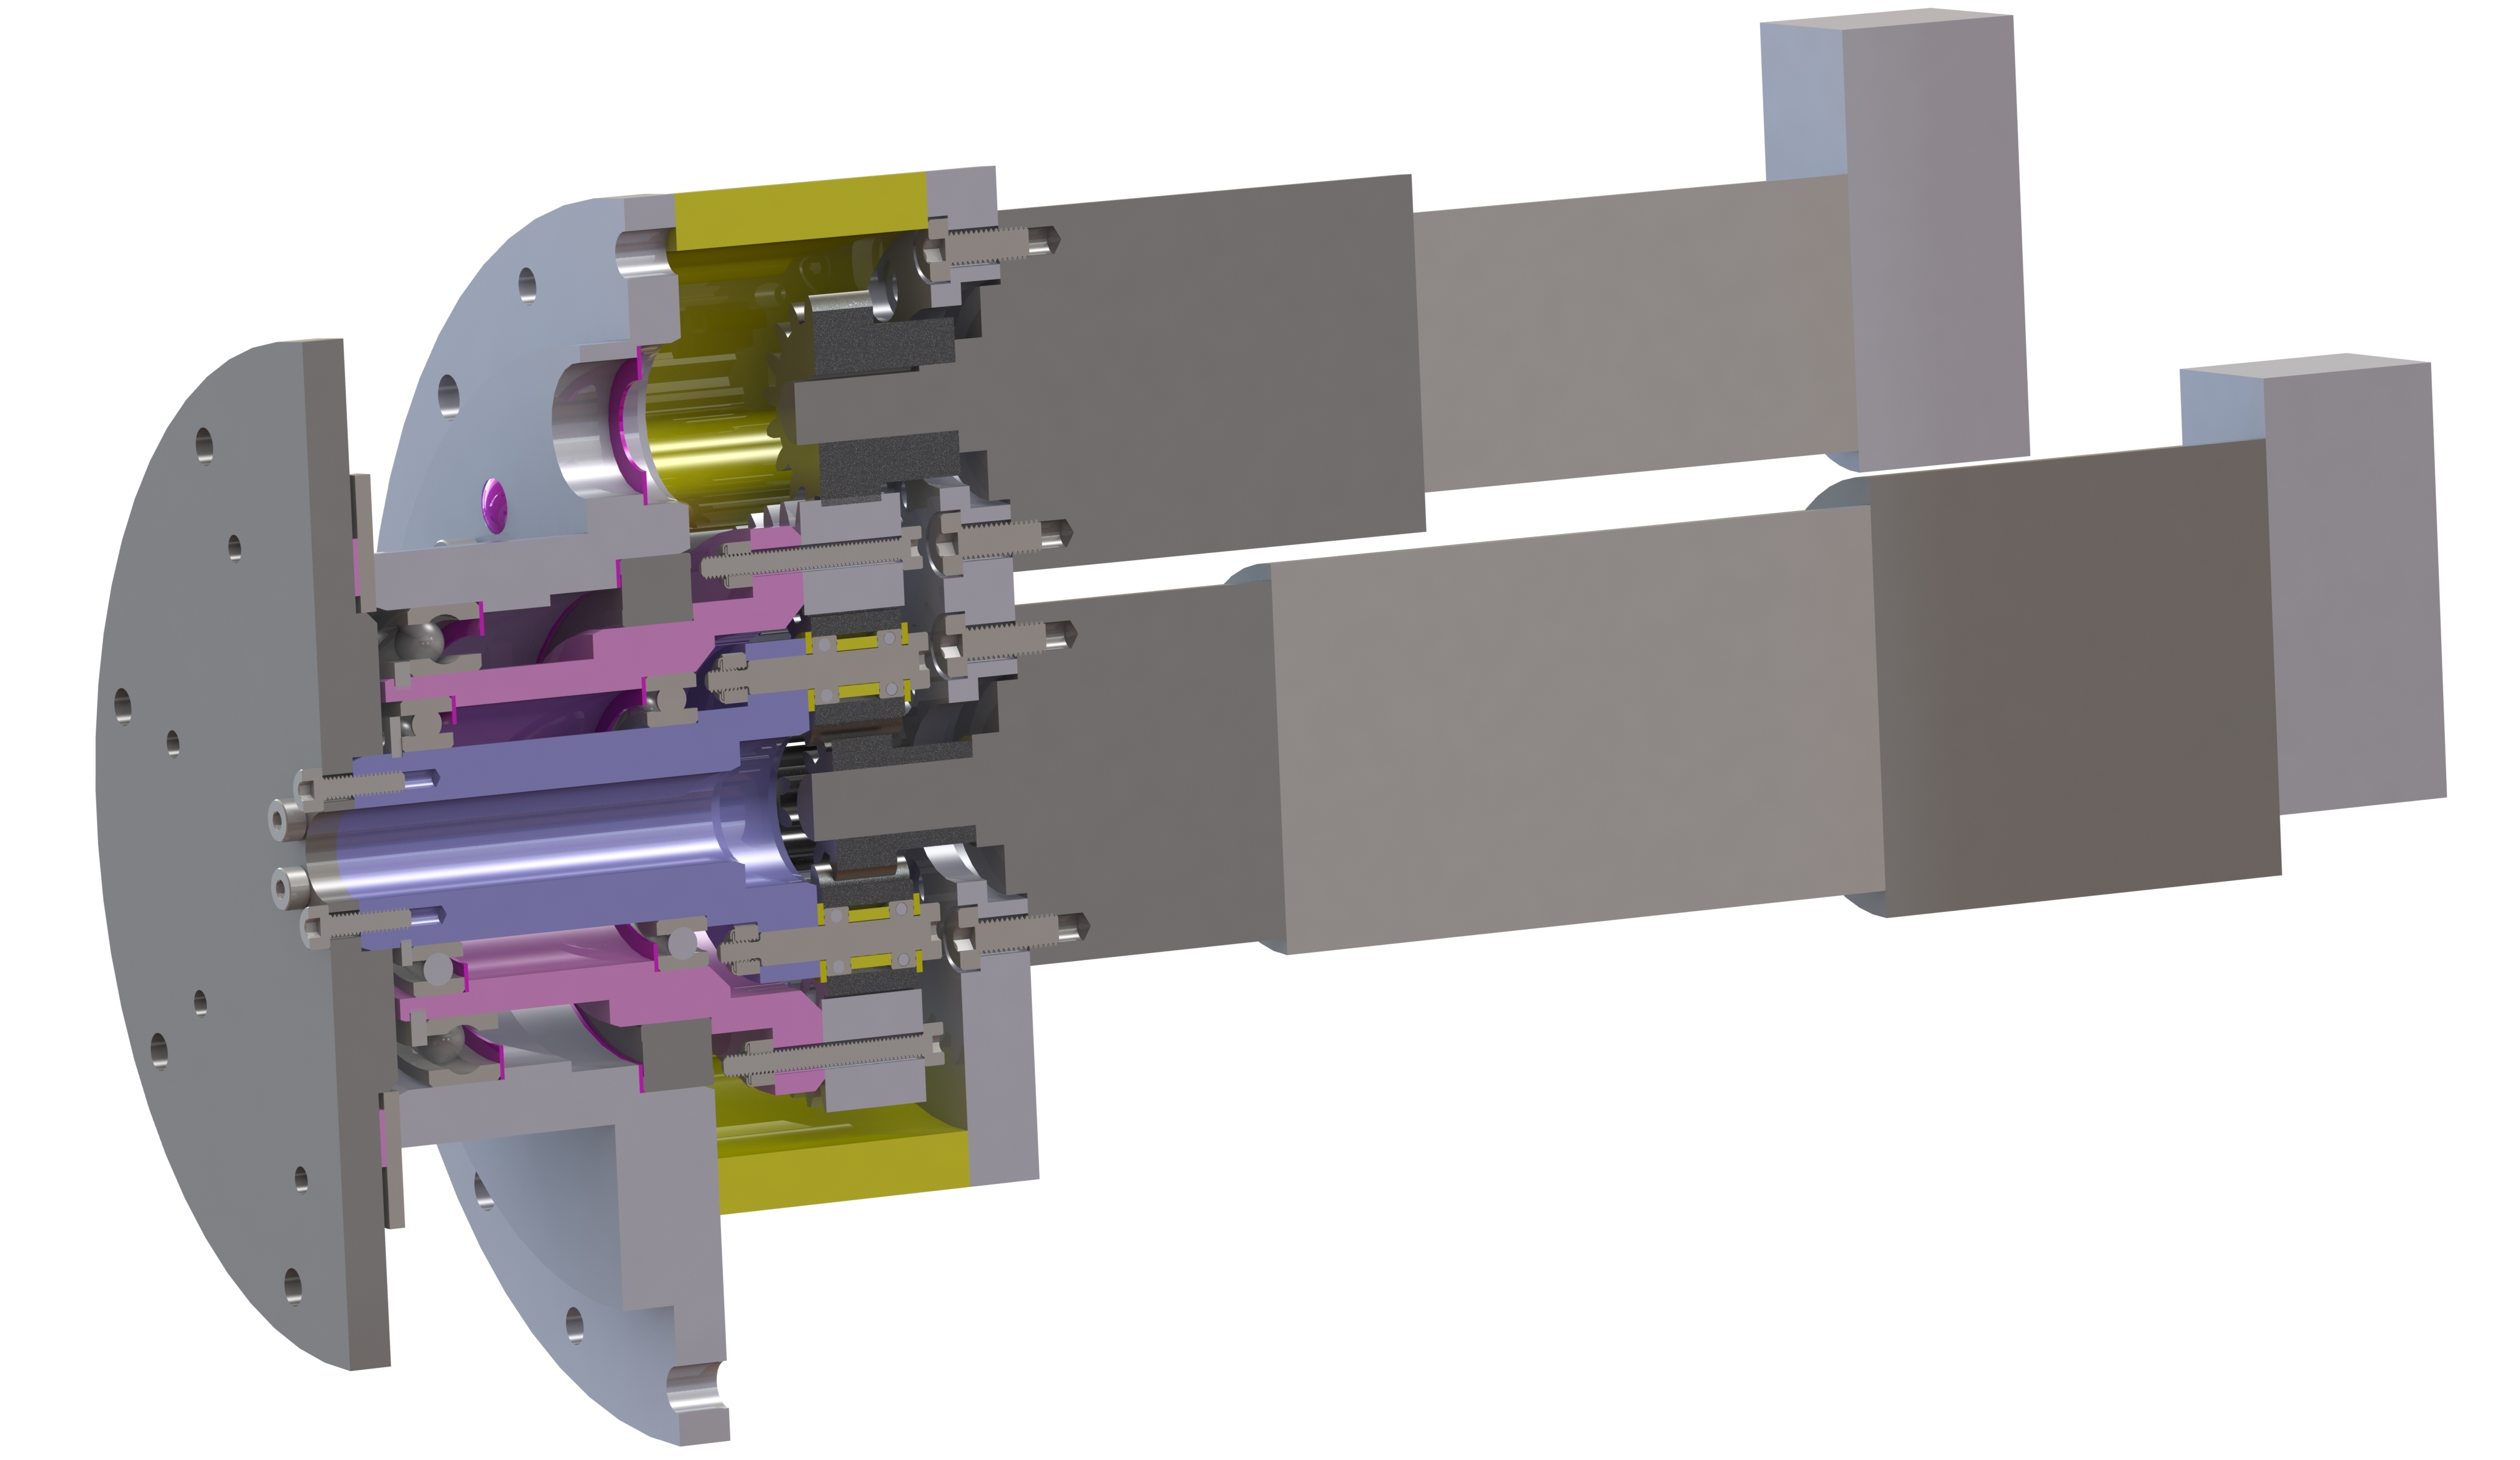
\includegraphics[width=0.95\textwidth]{metal_DSDM_section_view.jpg}
	\caption{Section view of the CAD model of the revolute actuator prototype} %Max continuous torque of 40 Nm and maximum velocity of 100 RPM
	\label{fig:dsdm_section}
\end{figure}

\begin{figure}[htbp]
	\centering
		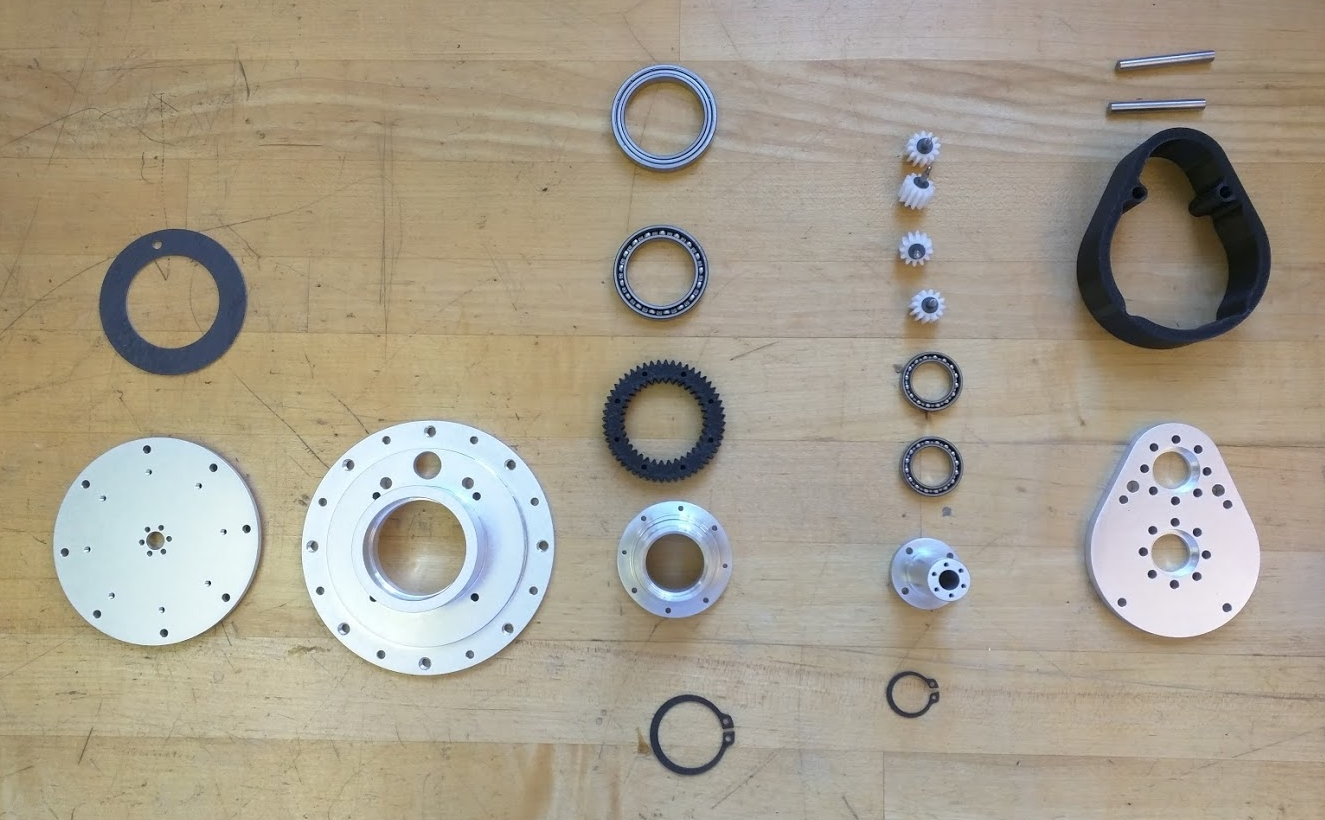
\includegraphics[width=0.90\textwidth]{dsdm_parts.jpg}
	\caption{Internal components of the revolute actuator prototype}
	\label{fig:dsdm_parts}
\end{figure}

A \textit{Maxon} motor of the serie RE-25, with maximum continuous power of 20 watts and torque 0.03 Nm, is used for M2, and motor of the serie RE-35, with maximum continuous power of 90 watts and torque 0.1 Nm, is used for M1. The revolute actuator prototypes use additional gear-head reduction for both motor, to increase both value of total reduction $R_1$ and $R_2$, to reach usefull range of torque and speeds, as illustrated at Table \ref{tab:specrev}. 
%
\begin{table}[htbp]
	\centering
	\caption{Specifications of revolute actuator prototypes}
		\begin{tabular}{ c c c c c c c}
			\hline
			Role & $R_1$ & $R_2$ & M1 power & M2 power & Max. Torque & Max. Velocity \\
			\hline
			       & $\frac{w_1}{w_o}$ & $\frac{w_2}{w_o}$ & Watts & Watts & Nm & RPM \\
			\hline \hline
			Elbow & 72 & 1225 & 100 & 20 & 37 & 70 \\
			Wrist & 23 & 474  & 100 & 20 & 15 & 220 \\
			\hline
		\end{tabular}
	\label{tab:specrev}
\end{table}
 
Note that the ratio $R_2/R_1$ is always keep at a factor of about 20, to match the capability of the brake according to eq. \eqref{eq:brakelim}. Also, the specifications of maximum torque, are given in term of very conservative continuous value advertized by \textit{Maxon} motor. Better performance could be obtained in term of peak torque during short time periods. The whole assembly of embeded DSDM actuator and support bearing for the revolute joint weight about 1.5 Kg. However, this value should not be taken as a state-of-art comparison reference to other actuation technology since 1) no optimization for weight has been conducted, 2) industrial DC \textit{Maxon} motor are don't have the best available power density and 3) the design was focus on ease of implementation and modularity. 


\subsubsection{Linear Actuator}

To achieve the large reduction needed for the shoulder actuator of the robot, while keeping the mechanism back-drivable during high-speed mode, a large-lead ballscrew linear stage is used. 

\begin{figure}[htp]
	\centering
		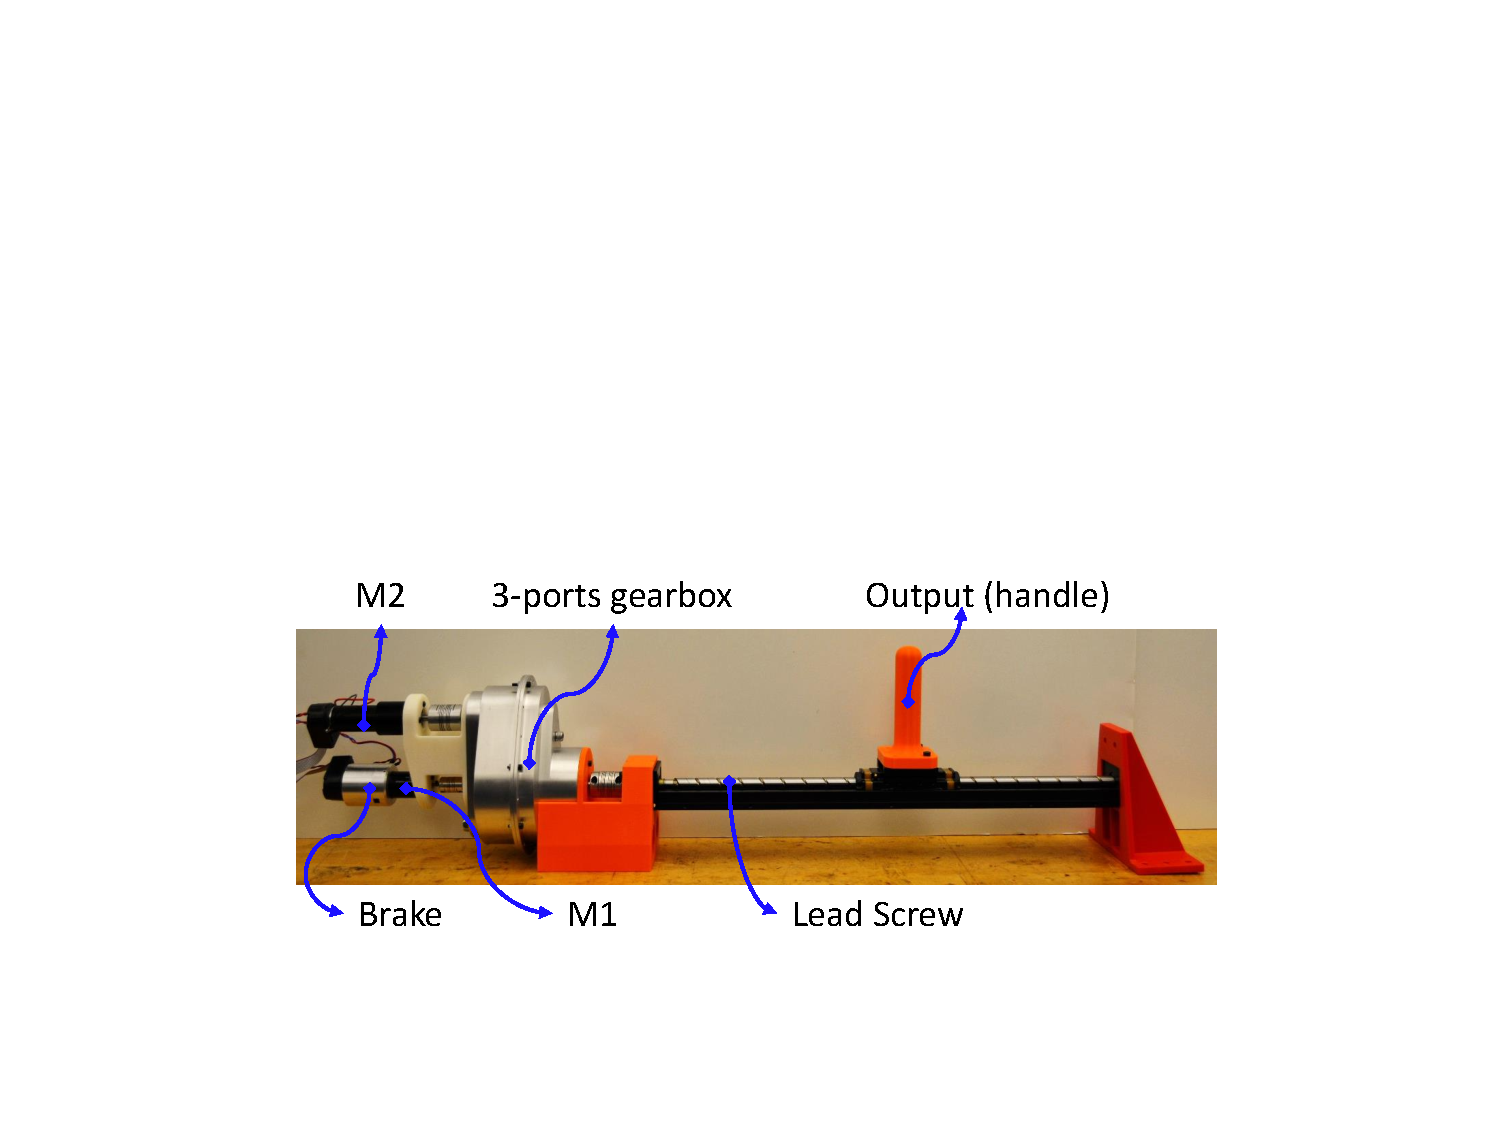
\includegraphics[width=0.95\textwidth]{proto_linear.pdf}
	\caption{linear actuator assembly} 
	\label{fig:linact}
\end{figure}

\begin{figure}[htbp]
	\centering
		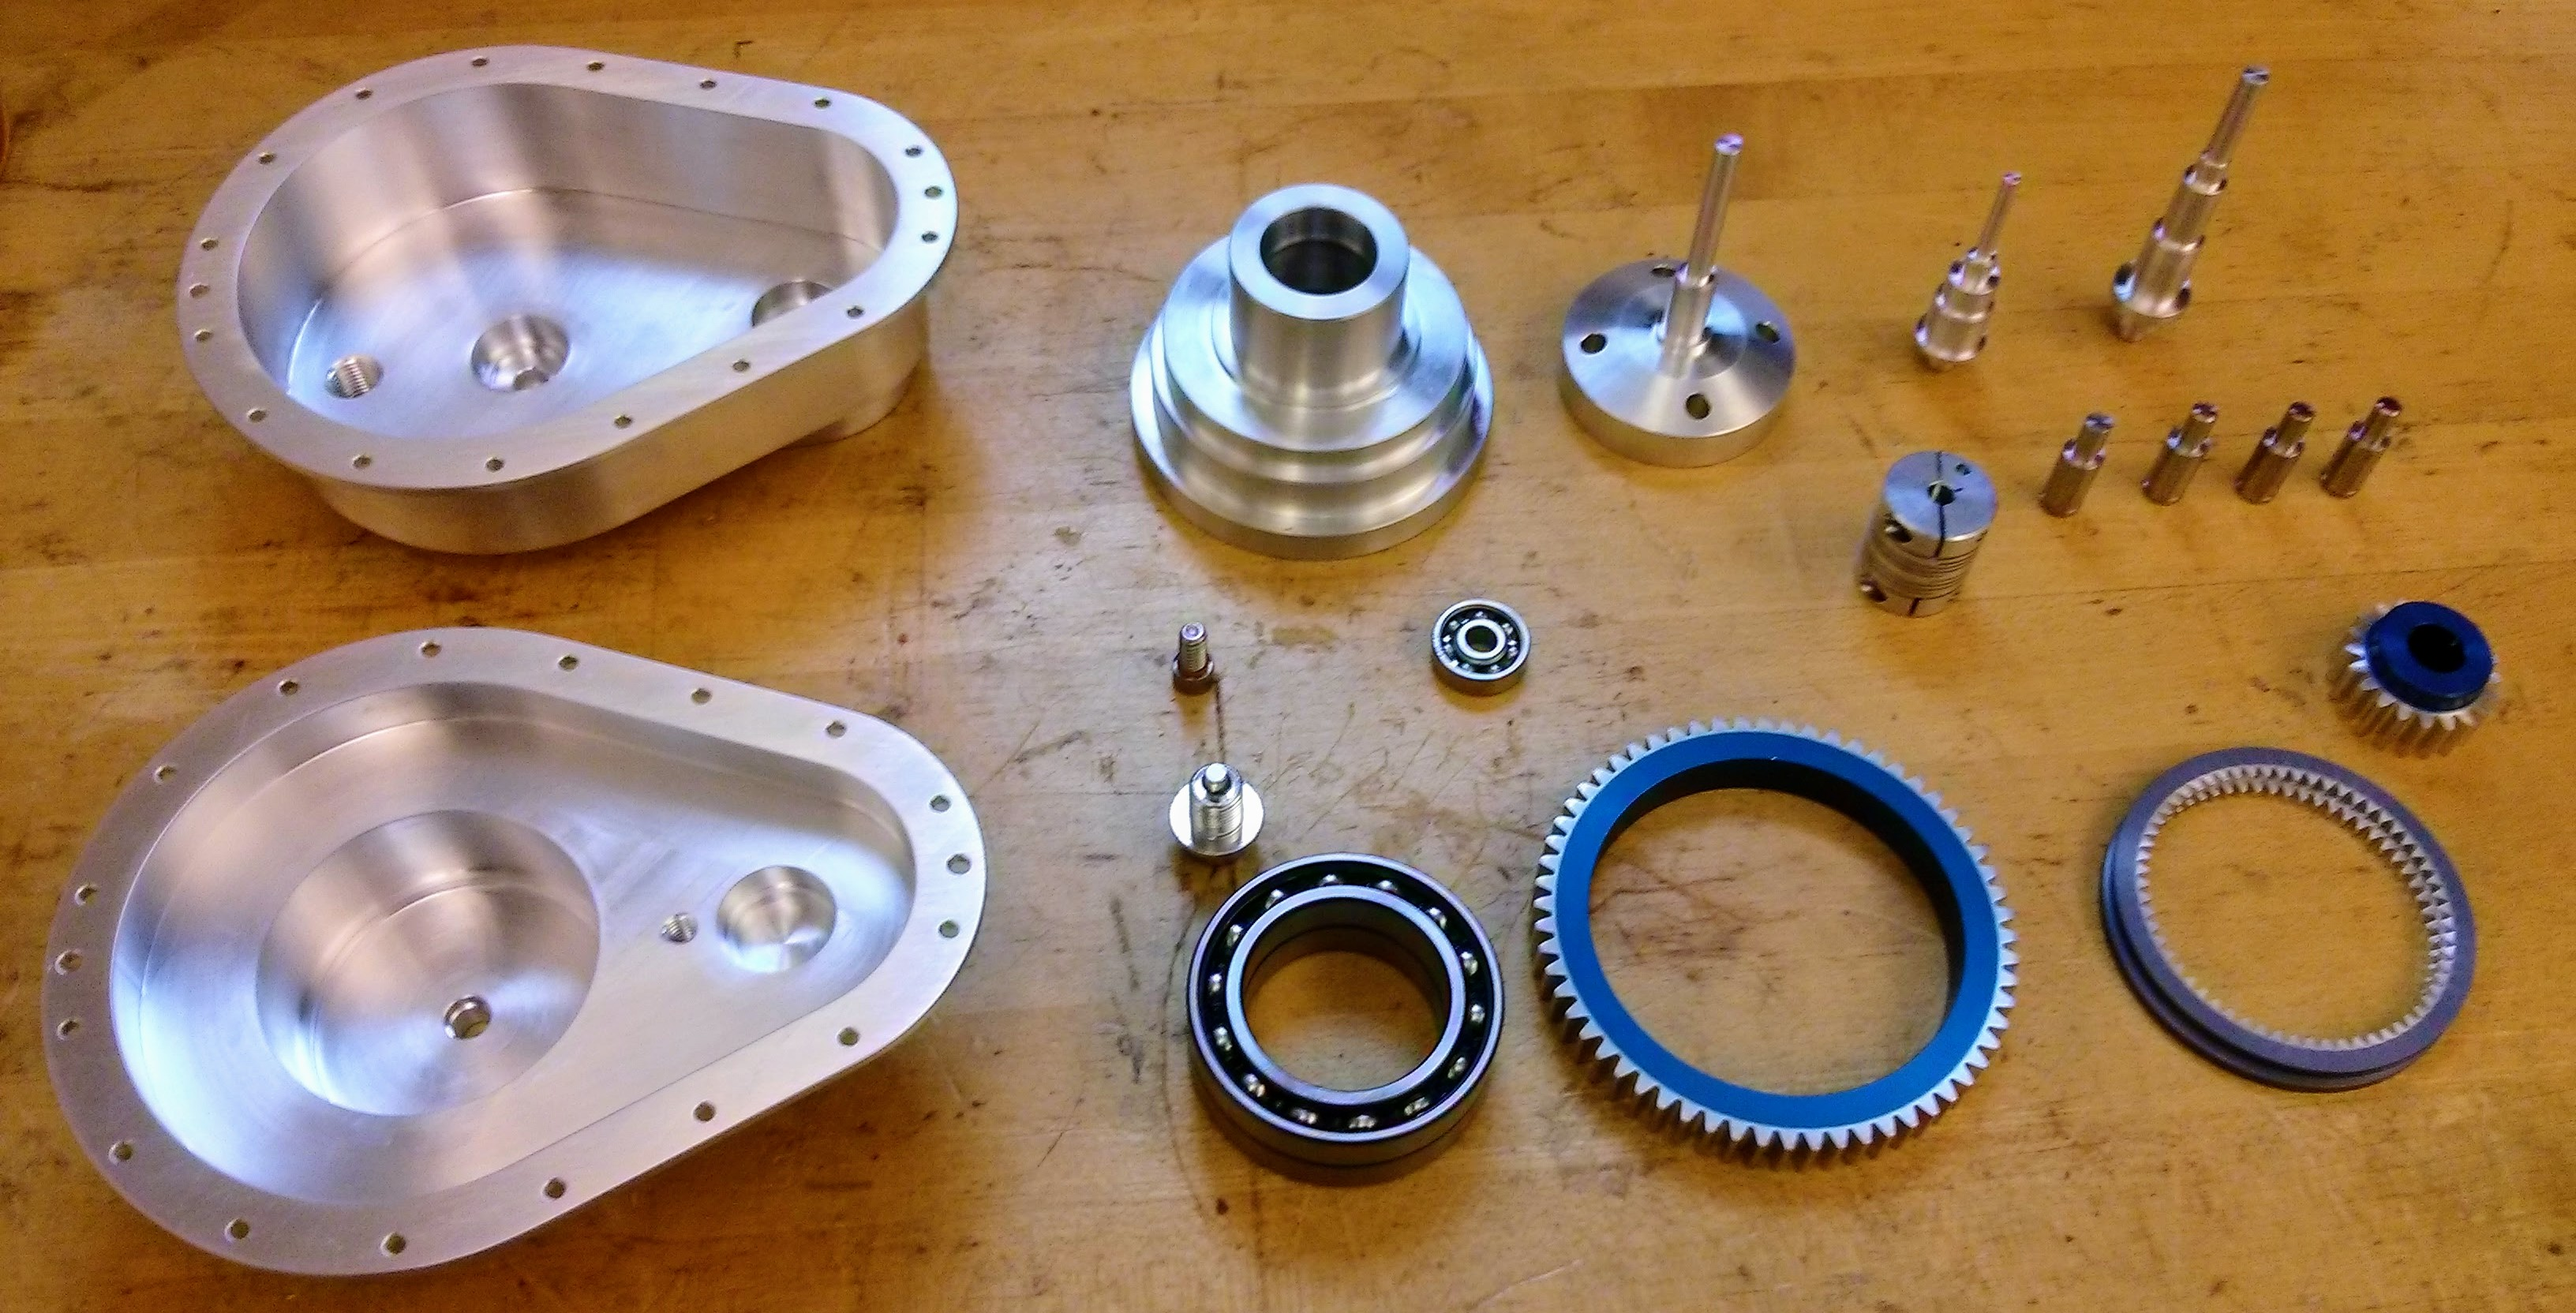
\includegraphics[width=0.90\textwidth]{dsdm_parts_old.jpg}
	\caption{Dsdm parts}
	\label{fig:dsdm_parts_old}
\end{figure}


\begin{table}[htbp]
	\centering
	\caption{Specifications of the linear actuator prototype}
		\begin{tabular}{ c c c c c c c c }
			\hline
			Role & $R_1$ & $R_2$ & Lead & M1 power & M2 power & Max. Force & Max. Velocity \\
			\hline
			       & $\frac{w_1}{w_o}$ & $\frac{w_2}{w_o}$ & mm/rev &Watts & Watts & N & m/s \\
			\hline \hline
			Shoulder & 4 & 72 & 20 & 20 & 20 & 600 & 0.7 \\
			\hline
		\end{tabular}
	\label{tab:specrev}
\end{table}


\subsection{Arm Design}
\label{sec:DSDMArm}

A custom robotic arm using 3 DSDM actuators was designed and built, see Fig. \ref{fig:dsdm_arm}. This arm is very strong and fast for its weight when compared to traditional robotic arms. 


\subsubsection{Shoulder 4-bar mechanism}

\begin{figure}[H]
	\centering
		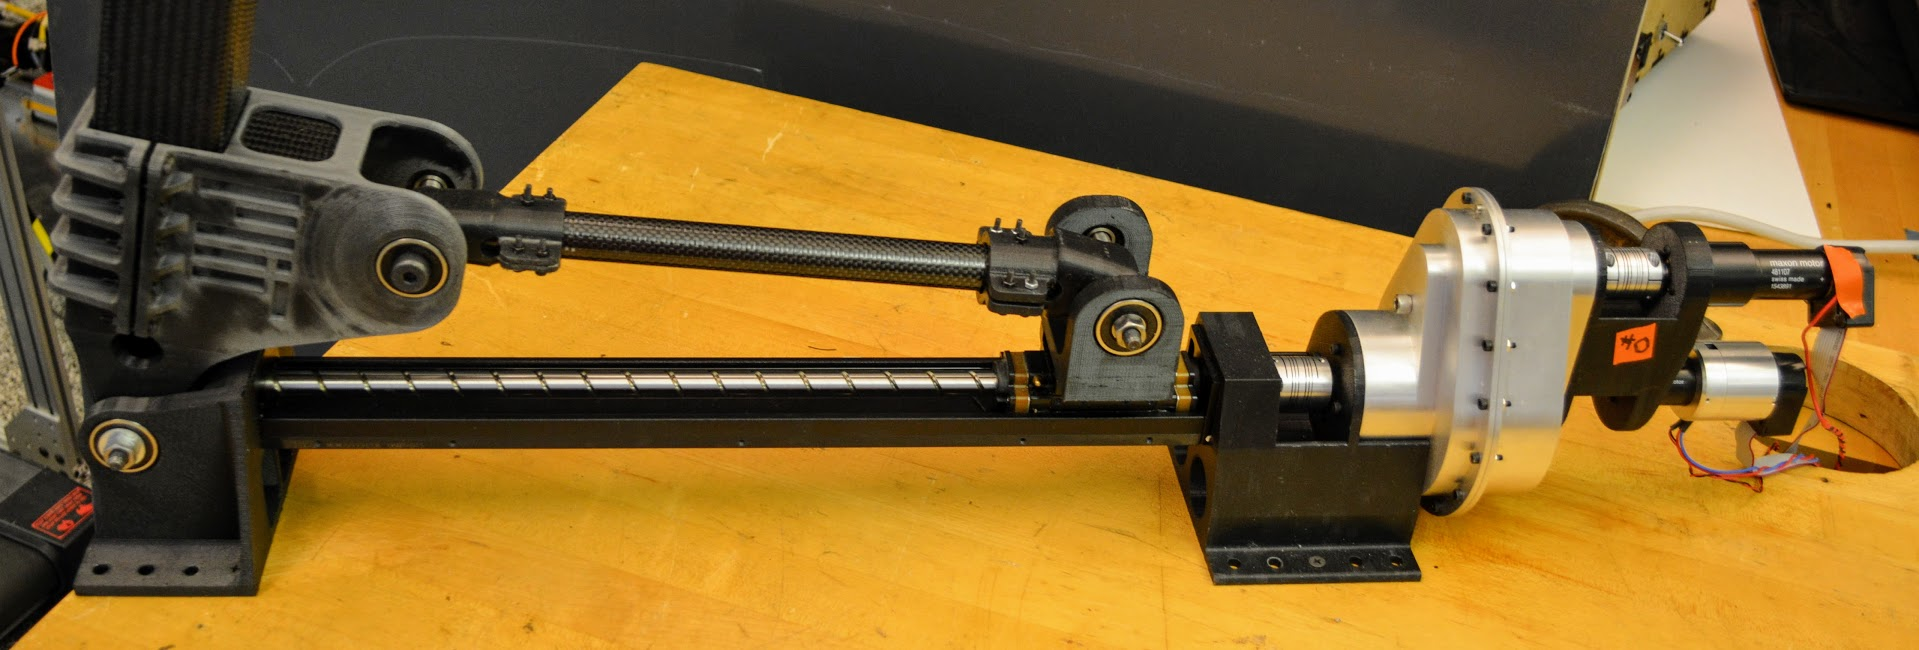
\includegraphics[width=0.95\textwidth]{4bar.jpg}
	\caption{Shoulder 4-bar mechanism}
	\label{fig:4bar}
\end{figure}



\section{Control and Software Architecture}
\label{sec:ControlSoftwareArchitecture}

\subsection{Architecture}

\begin{figure}[H]
	\centering
		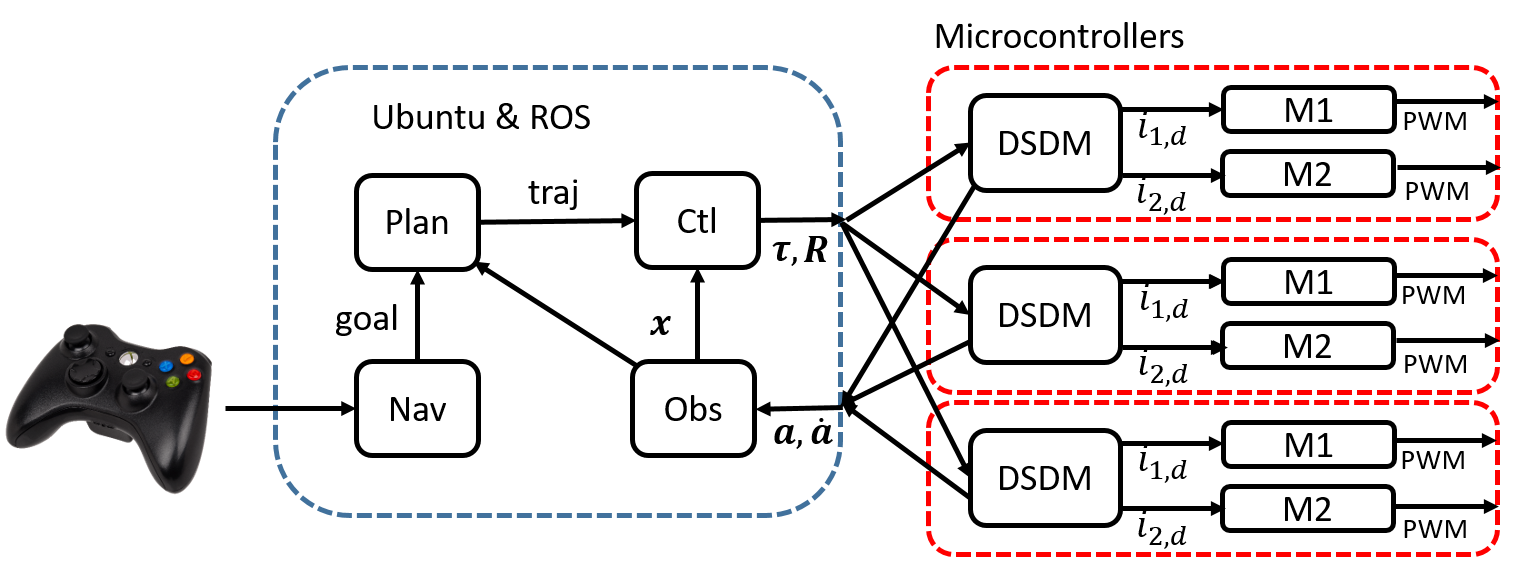
\includegraphics[width=0.95\textwidth]{ros_diagram.png}
	\caption{Control Software Architecture}
	\label{fig:ros_diagram}
\end{figure}


The control algorithms are implemented on a computer using ROS \cite{quigley_ros:_2009}, the trajectory generation algorithm and the R* Computed Torque controller are written in \textit{Python}. The computer is communicating over USB with open-source \textit{Flexsea} motor-drivers that handle the low-level current loops. The trajectory is generated offline in advance and loaded in memory upon initialization. The main R* control loop is running at a 500 Hz sampling rate. The low-level actuator controllers, receiving the torque and gear-ratio set-points, communicating with both motor drivers and handling the gear-shifting process (see Fig. \ref{fig:control_achitecture}), are ... TODO

%also implemented in \textit{Python} and use the algorithm described in \cite{girard_two-speed_2015}. Transition from one gear-ratio to another are found to be consistently under 50 ms.

\begin{figure}[H]
	\centering
		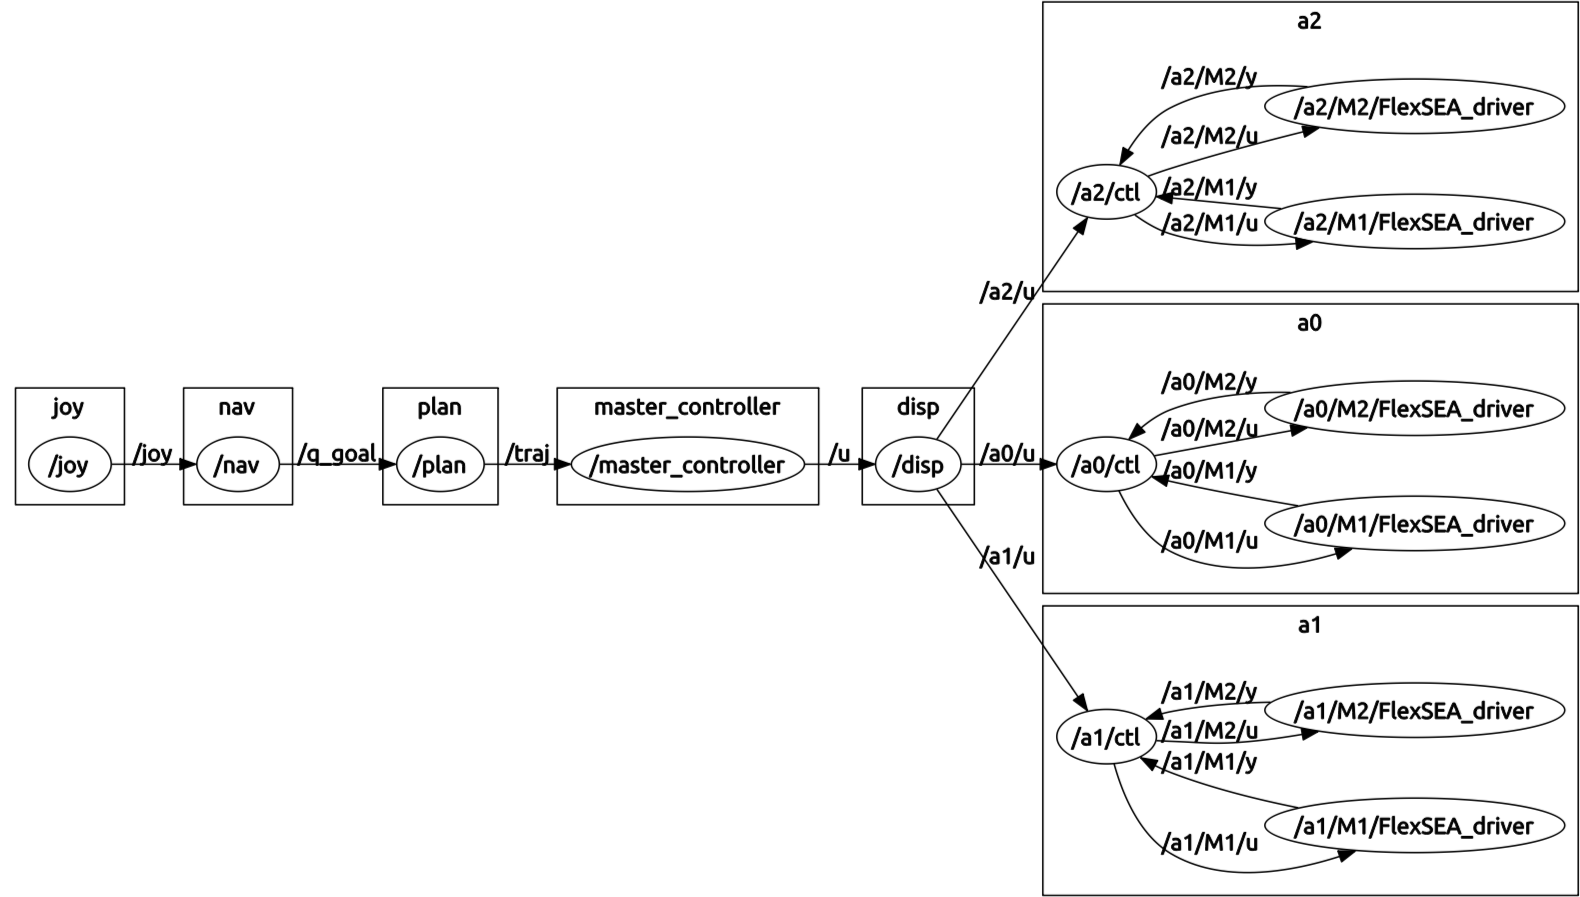
\includegraphics[width=0.95\textwidth]{ros_graph_3_dsdm.png}
	\caption{ROS architecture for controlling the full robot}
	\label{fig:ros_3dsdm}
\end{figure}


\begin{figure}[H]
	\centering
		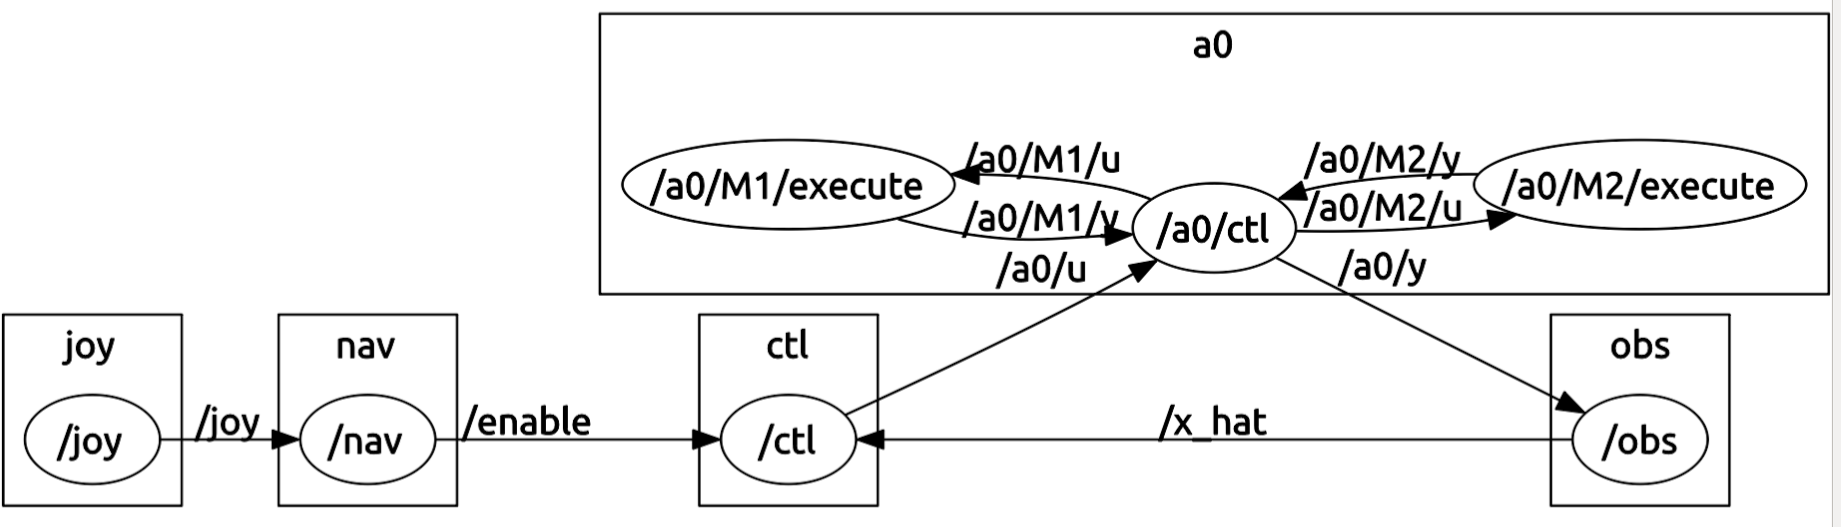
\includegraphics[width=0.95\textwidth]{ros_graph_single_dsdm.png}
	\caption{ROS architecture for controlling a single DSDM actuator directly}
	\label{fig:ros_dsdm}
\end{figure}


\subsection{Motor drivers}

The first generation NI Labview

Scaling to 6 motors and ROS connectivity

Second gen use micro-controllers \cite{duval_flexsea-execute:_2016} 

\subsection{DSDM Actuator Controllers}



\subsection{Robot Controller}

\subsection{Trajectory Planning }

